\documentclass[11pt]{article}
\usepackage[french]{babel}
\usepackage[utf8]{inputenc}
\usepackage[T1]{fontenc}
\usepackage{geometry}
\geometry{hmargin=2cm,vmargin=2cm}
\usepackage{eucal}
\usepackage{colortbl}
\usepackage{lscape}
\usepackage{amssymb}
\usepackage{amscd} 
\usepackage{amsfonts,amsmath,amsthm,amssymb,stmaryrd,eurosym} 
\usepackage{textcomp}
\usepackage{icomma}
\usepackage{calrsfs}
\usepackage{fancyhdr}
\usepackage{listings}
\usepackage{makecell}
\usepackage{graphicx}
\renewcommand{\v}[1]{\overrightarrow{#1}}
\usepackage[svgnames,dvipsnames]{xcolor}
\newcommand{\fboxb}[1]{\fbox{\color{blue}#1\color{black}}}
\renewcommand{\b}[0]{$\bullet$}
\usepackage{tcolorbox}
\usepackage{dirtree}

\definecolor{codegreen}{rgb}{0,0.6,0}
\definecolor{codegray}{rgb}{0.5,0.5,0.5}
\definecolor{codepurple}{rgb}{0.58,0,0.82}
\definecolor{backcolour}{rgb}{0.95,0.95,0.92}

\lstdefinestyle{mystyle}{
    backgroundcolor=\color{backcolour},   
    commentstyle=\color{codegreen},
    keywordstyle=\color{magenta},
    numberstyle=\tiny\color{codegray},
    stringstyle=\color{codepurple},
    basicstyle=\ttfamily\footnotesize,
    breakatwhitespace=false,         
    breaklines=true,                 
    captionpos=b,                    
    keepspaces=true,                 
    numbers=left,                    
    numbersep=5pt,                  
    showspaces=false,                
    showstringspaces=false,
    showtabs=false,                  
    tabsize=2,
    inputencoding=utf8,
    literate        =
                        {é}{{\'e}}{1}%
                        {è}{{\`e}}{1}%
}

\lstset{style=mystyle}




\title{Projet Pluridisciplinaire d'Informatique Intégrative}
\author{BEKHEDDA Maxence, GERMAIN Léo, GIANELLI Thomas, WALTER Théo}
\date{\today}
\begin{document}
\thispagestyle{empty}
\vspace*{-1.5cm}

\hspace{-1.5cm}\includegraphics[scale=0.2]{logo_tn.jpg}
	
\vspace*{-1.6cm}
	
\hspace{13.5cm}\includegraphics[scale=0.2]{logo_ul.png}



\vspace*{5cm}	% Espacement vertical
\begin{center}	% On centre le texte
{\Huge \bf PotaG \\\vspace{0.2cm} Le social en circuit court}\\	% \huge fait que le texte est gros, \bf fait que le texte est gras
\vspace{3cm}
\Large Projet Pluridisciplinaire d'Informatique Intégrative \\Recherche de solutions innovantes dans les circuits courts et les jardins partagés\\
\vspace{3cm}
Travail réalisé par BEKHEDDA Maxence,
GERMAIN Léo, \\GIANELLI Thomas et WALTER Théo
\vfill	% On va jusqu'au bas de la page avant de mettre le texte ci-dessous
\today
\end{center}
\newpage


\tableofcontents
\newpage
\section{Introduction}

Notre objectif était de créer une application mettant en relation des particuliers produisant des fruits et légumes en nombre trop important pour leur consommation personnelle avec des acheteurs intéressés par la consommation de produits locaux.

Nous avons alors réalisé une application divisée en deux parties principales. La première prend la forme d'un réseau social où les utilisateurs peuvent partager des photos de fruits et légumes, de potagers ou bien de plats cuisinés à partir de certains produits. La seconde partie est quant à elle un espace de vente où seuls les utilisateurs inscrits avec un profil de producteur peuvent y publier des annonces de vente de fruits et légumes. Ces annonces seront alors visibles par les utilisateurs inscrits sous un profil d'acheteur qui pourront désormais acheter les produits qui les intéressent.

Notre système de vente utilise des points relais, appelés \texttt{lockers}, disposés à plusieurs endroits en ville. Lorsqu'un utilisateur décide d'acheter un produit à un producteur, un algorithme détermine alors un casier dans lequel venir déposer et récupérer le produit acheté.

\begin{figure}[h]
    \centering
    \includegraphics[scale=0.33]{ScreenCasiers.png}
    \caption{Aperçu de la page \texttt{lockers} de notre application}
\end{figure}

\newpage

\section{L'application}
\subsection{Base de données}

L'utilisation de notre base de données est au coeur de notre application. Pour cela nous avons dû dans un premier temps réfléchir à une structure permettant de réaliser les fonctionnalités que nous voulions implémenter. Nous avons alors établi le shéma relationnel\footnote{Les cardinalités des  associations ne sont pas correctes sur ce graphique} suivant:

\begin{figure}[h]
\begin{center}
\includegraphics[scale=0.46]{DiagrammeBD.png}
\caption{Schéma relationnel de la première version de notre base de données}
\end{center}
\end{figure}

Néanmoins, au fur et à mesure que nous implémentions des fonctionnalités dans notre application, nous avons réalisé que notre base de données ne permettait pas d'obtenir les résultats désirés.

Nous avons fait évoluer la base de données afin qu'elle réponde au mieux à nos besoin. La base de donnée obtenue est détaillée ci-dessous.
\vspace{0.4cm}

Notre nouvelle base de données se compose de 8 tables:
\begin{itemize}
    \item Producteur
    \item Acheteur
    \item Social
    \item Casier
    \item Follow
    \item Like
    \item File\_attente
    \item Transaction
\end{itemize}
\vspace{0.4cm}

Toutes ces tables ont été créées grâce à un programme Python et au module \texttt{sqlite3}. Voici un extrait de code nous ayant permis de générer la base de données:

\begin{lstlisting}[language=Python, caption={Code Python permettant de créer la table \texttt{producteur}}]
con = sqlite3.connect("../potag_main.db")
cur = con.cursor()

cur.execute("CREATE TABLE producteur ( \
    id_producteur VARCHAR(100) PRIMARY KEY, \
    nom VARCHAR(40), \
    prenom VARCHAR(40), \
    mail VARCHAR(100), \
    password VARCHAR(100), \
    profile VARCHAR(100), \
    adresse_producteur VARCHAR(40), \
    ville_producteur VARCHAR(40), \
    casier INT );")
\end{lstlisting}
\subsubsection{Utilisateurs}

Les tables \texttt{producteur} et \texttt{acheteur} sont construites de manière identique. Selon le profil que l'utilisateur renseigne lors de la création de son compte, il sera enregistré dans l'une des deux. La clé primaire de ces deux tables est l'\texttt{id\_acheteur} (ou \texttt{id\_producteur}). Il correspond au nom d'utilisateur qui a été choisi, sachant que pour celui-ci soit unique, un test est réalisé à l'inscription. Le \texttt{nom} et le \texttt{prénom} de l'utilisateur sont également renseignés à l'inscription sans contraintes particulières. L'adresse mail de l'utilisateur est elle aussi ajoutée à la colonne \texttt{mail} lors de l'inscription, à condition qu'elle respecte le format suivant exemple@nom.domaine (exemple, nom et domaine doivent contenir au minimum un caractère). Ensuite, le mot de passe est enregistré dans la colonne \texttt{password}. Pour cela, il doit respecter 4 conditions: être de plus de 8 caractères, contenir au moins une majuscule, une minuscule et un chiffre. La colonne \texttt{profile} contiendra quant à elle le chemin vers la photo de profil de l'utilisateur. Ce champ peut être rempli ou non par l'utilisateur, tout comme son adresse et sa ville. Enfin, la colonne \texttt{casier} est remplie dans le cas d'une transaction. Elle contient pour le producteur ou pour l'acheteur l'identifiant du casier dans lequel il doit aller déposer ou récupérer ces produits. 

\subsubsection{Social}

 Ensuite vient la table \texttt{social}, qui permet d'accéder à toutes les publications faites par les utilisateurs.
 
 \begin{figure}[h]
     \centering
     \includegraphics[scale=0.6]{SocialBDExemple.png}
     \caption{Exemple de contenu dans la table \texttt{social}}
 \end{figure}

La première colonne est la clé primaire, c'est l'identifiant de la publication. Il est ajouté de manière automatique à chaque fois qu'une image est publiée grâce à la fonction \texttt{AUTOINCREMENT}. L'\texttt{id\_auteur} correspond à l'\texttt{id\_acheteur} de l'utilisateur ayant fait la publication. La date et l'heure sont elles aussi ajoutées automatiquement et correspondent au moment auquel l'utilisateur publie son post. Le \texttt{contenu\_post} contient une description en moins de 300 caractères que l'utilisateur a choisi d'associer à sa photo. Enfin le \texttt{lien\_image} correspond au chemin d'accès à la photo publiée.
\vspace{0.4cm}

La table \texttt{follow} est extrêmement simple mais elle nous est très pratique. À chaque fois qu'un utilisateur (le \texttt{follower}) décide de suivre le profil d'un autre utilisateur (le \texttt{followed}), une ligne est ajoutée dans la table. Cela nous permet alors d'accéder facilement à notre nombre de followers, ou bien à la liste des profils que l'on suit.

\begin{lstlisting}[language=SQL, caption={Exemple de requete SQL sur la table \texttt{follow}}]
COUNT * FROM follow WHERE followed = Thomas; --compte le nombre de followers de Thomas
SELECT followed FROM follow WHERE follower = Maxence; --renvoie les profils suivie par Maxence
\end{lstlisting}
\vspace{0.4cm}

La table \texttt{like} est elle aussi très simple. Lorsque un utilisateur "like" un post, une ligne est ajoutée avec l'\texttt{id\_post} (l'identifiant unique de la publication) et l'\texttt{id\_liker} (le nom d'utilisateur ayant aimé la publication). Grâce à cette table, on peut alors savoir facilement combien de fois une publication a été likée ou combien de publications ont été likées par un utilisateur.

 
\begin{figure}[h]
    \centering
    \includegraphics[scale=0.65]{LikeBDExemple.png}
    \caption{Exemple de contenu dans la table \texttt{like}}
\end{figure}

Dans cet exemple, la publication numéro 3 a été likée deux fois, et l'utilisateur Théo a aimé trois publications.

\subsubsection{Ventes}

La table \texttt{transactions} présente de nombreuses similitudes avec la table \texttt{social}, elle est en quelque sorte son équivalent pour les producteurs. En effet, les producteurs ont la possibilité de faire des publications, mais celles-ci apparaissent dans un onglet séparé et sont accompagnées d'un prix. C'est pour cette raison qu'en plus de reprendre les colonnes de la table \texttt{social}, une colonne \texttt{prix\_produit} est ajoutée, contenant le prix en euros de l'article mis en vente. De plus cette table comprend également une colonne \texttt{vendu} qui indique si un produit a été vendu ou pas encore.

\begin{lstlisting}[language=Python, caption={Code Python permettant de créer la table \texttt{transaction}}]
cur.execute("CREATE TABLE transactions ( \
    id_transaction INTEGER PRIMARY KEY AUTOINCREMENT, \
    id_producteur VARCHAR(20) REFERENCES Producteur(id_producteur), \
    lien_image VARCHAR(100), \
    date_offre DATE, \
    prix_produit FLOAT(7), \
    description VARCHAR(200), \
    vendu VARCHAR(100) );")
\end{lstlisting}
    
La table \texttt{casier} est au coeur de notre système de vente. Sa taille est fixe, elle contient 396 lignes. Tous nos points de vente se trouvent à Nancy, et ils sont au nombre de 18. Dans chacun de ces points de vente, nous avons considéré qu'il y a 22 casiers; d'où les 396 lignes: une par casier. À chaque casier est affecté un identifiant unique, une adresse, la ville dans laquelle il se trouve (dans notre cas c'est toujours Nancy), et un nombre de 0 à 21 unique à chaque point de vente. Enfin, une dernière colonne indique grâce à un booléen si le casier est actuellement utilisé, ou s'il est libre.

\begin{figure}[h]
	\centering
	\includegraphics[scale=0.6]{CasierBDExemple.png}
	\caption{Extrait de la table \texttt{casiers}}
\end{figure}
On peut voir un casier vide et deux casiers pleins au point de vente 0 du 15 Avenue Anatole France ainsi que deux casiers vides au point de vente 1 situé au 118 Avenue de Boufflers.
\vspace{0.4cm}

La table \texttt{file\_attente} permet de savoir quels produits ont été achetés. Lorsqu'un utilisateur achète un produit, on insère dans la colonne \texttt{acheteur} le nom de l'utilisateur et dans la colonne \texttt{vendeur}, le nom du producteur ayant mis en vente le produit. On considère donc qu'un acheteur ne peut acheter qu'un produit à la fois, et que de même, un producteur ne peut vendre qu'un produit à la fois.


\subsection{Serveur web}
Notre serveur web fonctionne avec le framework Flask en python. Avec Flask, on peut accéder à des pages html dynamiques. Pour cela on utilise des fonctions python qui renvoient les fichiers html avec des variables. L’arboresence du projet est la suivante:
\dirtree{%
.1 web\_app.
.2 database.
.3 potag\_main.db.
.2 static.
.3 css.
.4 ....
.3 images.
.4 ....
.3 script.
.4 script.js.
.2 templates.
.3 layout.
.4 base.html.
.4 base\_login.html.
.3 achats.html.
.3 ....
.2 test\_algo.
.3 test\_1.py.
.3 ...
.2 venv.
.3 ....
.2 algo.py.
.2 app.py.
.2 outils.py.
.2 potag\_login.py.
.2 potag\_preferences.py.
.2 requirements.txt.
.2 potag\_social.py.
.2 potag\_vente.py.
}
\vspace{0.4cm}

Le serveur web fonctionne avec un fichier flask\_app: \texttt{app.py}. 
Pour ne pas avoir toutes les fonctions dans le fichier \texttt{app.py}, les fonctions sont séparées dans 6 fichiers python en fonction de leurs utilisations:

\begin{itemize} 
\item algo.py
\item outils.py
\item potag\_login.py
\item potag\_social.py
\item potag\_vente.py
\item potag\_preferences.py
\end{itemize} 

On importe ces 6 modules dans \texttt{app.py}.

\subsubsection{app.py}

L'app.py est celle lancée pour faire fonctionner le serveur web. Depuis le module flask, on importe Flask qui permet de configurer le serveur.
\begin{lstlisting}[language=Python, caption={Code Python permettant de configurer le serveur}]
app = Flask(__name__)
app.config['SECRET_KEY'] = 'UneCléSecrète'
app.config["SESSION_PERMANENT"] = False
app.config["SESSION_TYPE"] = "filesystem"
app.config['UPLOAD_FOLDER'] = 'static/images/'

\end{lstlisting}

Il faut ensuite déclarer les routes à flask. Elles sont rangées en 4 catégories: login, social, ventes et préférences.

\begin{lstlisting}[language=Python, caption={Code Python permettant de déclarer la route \texttt{login} et \texttt{publications}}]
# Login
import potag_login
app.add_url_rule('/login', view_func=potag_login.login,methods=["POST", "GET"]
...

# Social
import potag_social
app.add_url_rule('/publications', view_func=potag_social.publications,methods=["POST", "GET"]
...
\end{lstlisting}

Dans l'exemple précédent, la première route concernée est /login et la fonction correspondante est potag\_login.login(). 
L'appel à une route sur le navigateur lance la fonction python associé.
On remarque que les fonctions sont importées depuis les modules cités précédemment.
Les informations de connexion sont enregistrées grace au module \texttt{flask.session}.

\begin{lstlisting}[language=Python, caption={Code Python permettant d'ajouter un élément dans session}]
session["name"]="Didier"
session["compte"]="producteur"
\end{lstlisting}

\subsubsection{potag\_login.py}

C'est dans ce module que sont regroupées toutes les fonctions liées à la connexion:
\begin{itemize} 
\item \texttt{signup()} pour s’inscrire 
\item \texttt{passwordchoice()} pour choisir un mot de passe
\item \texttt{login()} pour se connecter
\item \texttt{password()} pour indiquer le mot de passe de connexion
\item \texttt{logout()} pour se déconnecter
\item \texttt{forgot()} en cas d'oubli de mot de passe
\end{itemize} 
\vspace{0.4cm}

Elles permettent de créer un compte et de se connecter. Prenons comme exemple la fonction login().
\begin{lstlisting}[language=Python, caption={Fonction Python \texttt{login}}]
def login():
    session.clear()
    if request.method == "POST":
        session["name_temp"] = corrige_espace(request.form.get("name"))
        db=sqlite3.connect(DATABASE)
        cursor=db.cursor()
        cursor.execute("SELECT id_acheteur FROM acheteur WHERE id_acheteur= ?", (session["name_temp"], ))
        login=cursor.fetchall()
        if login==[]:
            cursor.execute("SELECT id_producteur FROM producteur WHERE id_producteur= ?", (session["name_temp"], ))
            session["compte"]="producteur"
        else:
            session["compte"]="acheteur"
        db.close()
        return redirect("/password")
    return render_template("login.html")
\end{lstlisting}

Pour pouvoir afficher la page html il nous faut le module \texttt{flask.render\_template}. Notre fonction retourne donc render\_template("login.html") ce qui permet de renvoyer le fichier html. En cas de requête POST, c'est-à-dire quand on clique sur "valider", on ajoute la donnée de "nom d'utilisateur" dans session. On détermine si c'est un acheteur ou un producteur puis on ajoute l’information dans session. Enfin, on redirige vers /password. On interroge la base de donnée grâce au module \texttt{sqlite3}. Les pages html, qui sont dans templates/, viennent s'ajouter à \texttt{base\_login.html} qui se trouve dans templates/layout/. Elles utilisent \texttt{inscription.css} dans static/css/.


\begin{figure}[h]
    \centering
    \includegraphics[scale=0.4]{ScreenLogin.png}
    \caption{Formulaire de la page \texttt{login.html}}
\end{figure}

\subsubsection{potag\_social.py}

C'est dans ce module que sont regroupées toutes les fonctions liées à la partie réseau social de notre application:

\begin{itemize} 
\item \texttt{publications()} pour voir les publications d'autres utilisateurs
\item \texttt{publicationliked()} pour voir les publications likées
\item \texttt{addpublication()} pour publier une image
\item \texttt{profil()} pour voir son profil
\item \texttt{deletepost()} pour supprimer une publication
\item \texttt{visitprofile(username)} pour voir le profil d'autres utilisateurs
\item \texttt{profilsfollowed()} pour voir les profils suivis
\item \texttt{followers()} pour voir les profils qui nous suivent
\item \texttt{recherche()} pour effectuer une recherche
\end{itemize} 
\vspace{0.4cm}

Prenons comme exemple la fonction publications. C'est une fonction assez lourde car elle permet l'affichage des publications de chaque utilisateur accompagnées de leurs likes.

\begin{lstlisting}[language=Python, caption={Fonction Python \texttt{publications}}]
def publications():
    active=recup_infos()
    if not active:
        return redirect('/')
    info=session["infos_perso"]
    if request.method=="POST":
        idpost=request.form.get("idpost")
        db = sqlite3.connect(DATABASE)
        cursor= db.cursor()
        cursor.execute("SELECT id_post FROM like WHERE (id_post, id_liker) = (?, ?)", (idpost, session["name"]))
        res=cursor.fetchall()
        if len(res)>0:
            cursor.execute("DELETE FROM like WHERE (id_post, id_liker) = (?, ?)", (idpost, session["name"]))
        else:
            cursor.execute("INSERT INTO like (id_post, id_liker) VALUES (?, ?)", (idpost, session["name"]))
        db.commit()
        db.close()
    db = sqlite3.connect(DATABASE)
    cursor= db.cursor()
    cursor.execute("SELECT id_post, id_auteur, lien_image, contenu_post, date_post, heure_post FROM social ORDER BY date_post")
    posts_temp=cursor.fetchall()
    posts=[]
    for post in posts_temp:
        post = list(post)
        cursor.execute("SELECT count(id_liker) from like where id_post=?;",[post[0]])
        likes = cursor.fetchall()[0][0]
        post.append(likes)
        cursor.execute("SELECT id_post FROM like WHERE (id_post, id_liker) = (?, ?)", (post[0], session["name"]))
        res=cursor.fetchall()
        if len(res)>0:
            post.append("true")
        else:
            post.append("false")
        posts.append(post)
    db.close
    posts.reverse()
    return render_template("publications.html", compte=info, posts=posts)
\end{lstlisting}

On remarque tout d'abord l'utilisation de outils.recup\_info qui permet, en plus d'ajouter les informations de l'utilisateur dans session, de vérifier que l'utilisateur est connecté. En effet si session["name"] n'existe pas alors recup\_info renvoie False et on est renvoyé vers /login. Ce test est réalisé dans chaque fonction car il évite toutes les erreurs liées à une personne non connectée. Si l'utilisateur était bien connecté, on récupère des infos sur son profil dans la variable \texttt{info}.

Si une requête de type \texttt{POST} est effectuée sur la page, c'est que le bouton de "like" a été cliqué par l'utilisateur. Il existe alors deux cas de figure:
\begin{itemize}
    \item La publication était déjà likée, l'utiliasteur veut donc retirer son like,
    \item La publication n'était pas likée, l'utilisateur vient donc de la liker.
\end{itemize}

Pour savoir dans quel cas nous sommes, il nous faut vérifier si la base de données contient le like entre l'utilisateur et la publication en question. Puis selon la situation, il nous faut alors ajouter ou supprimer cette ligne dans la table \texttt{like}.

Dans tous les cas, la page doit afficher les publications. On effectue donc une requête dans la base de données pour récuperer toutes les informations de toutes les publications, que l'on trie par ordre chronologique. Pour chacune de ces publications, on va ensuite calculer combien de fois elles ont été likées et si elles sont likées par l'utilisateur connecté. Une fois toutes ces informations relevées, on retourne la page \texttt{publications.html} en affichant les publications par ordre antichronologique pour voir les publications les plus récentes en premier.

\begin{figure}[h]
    \centering
    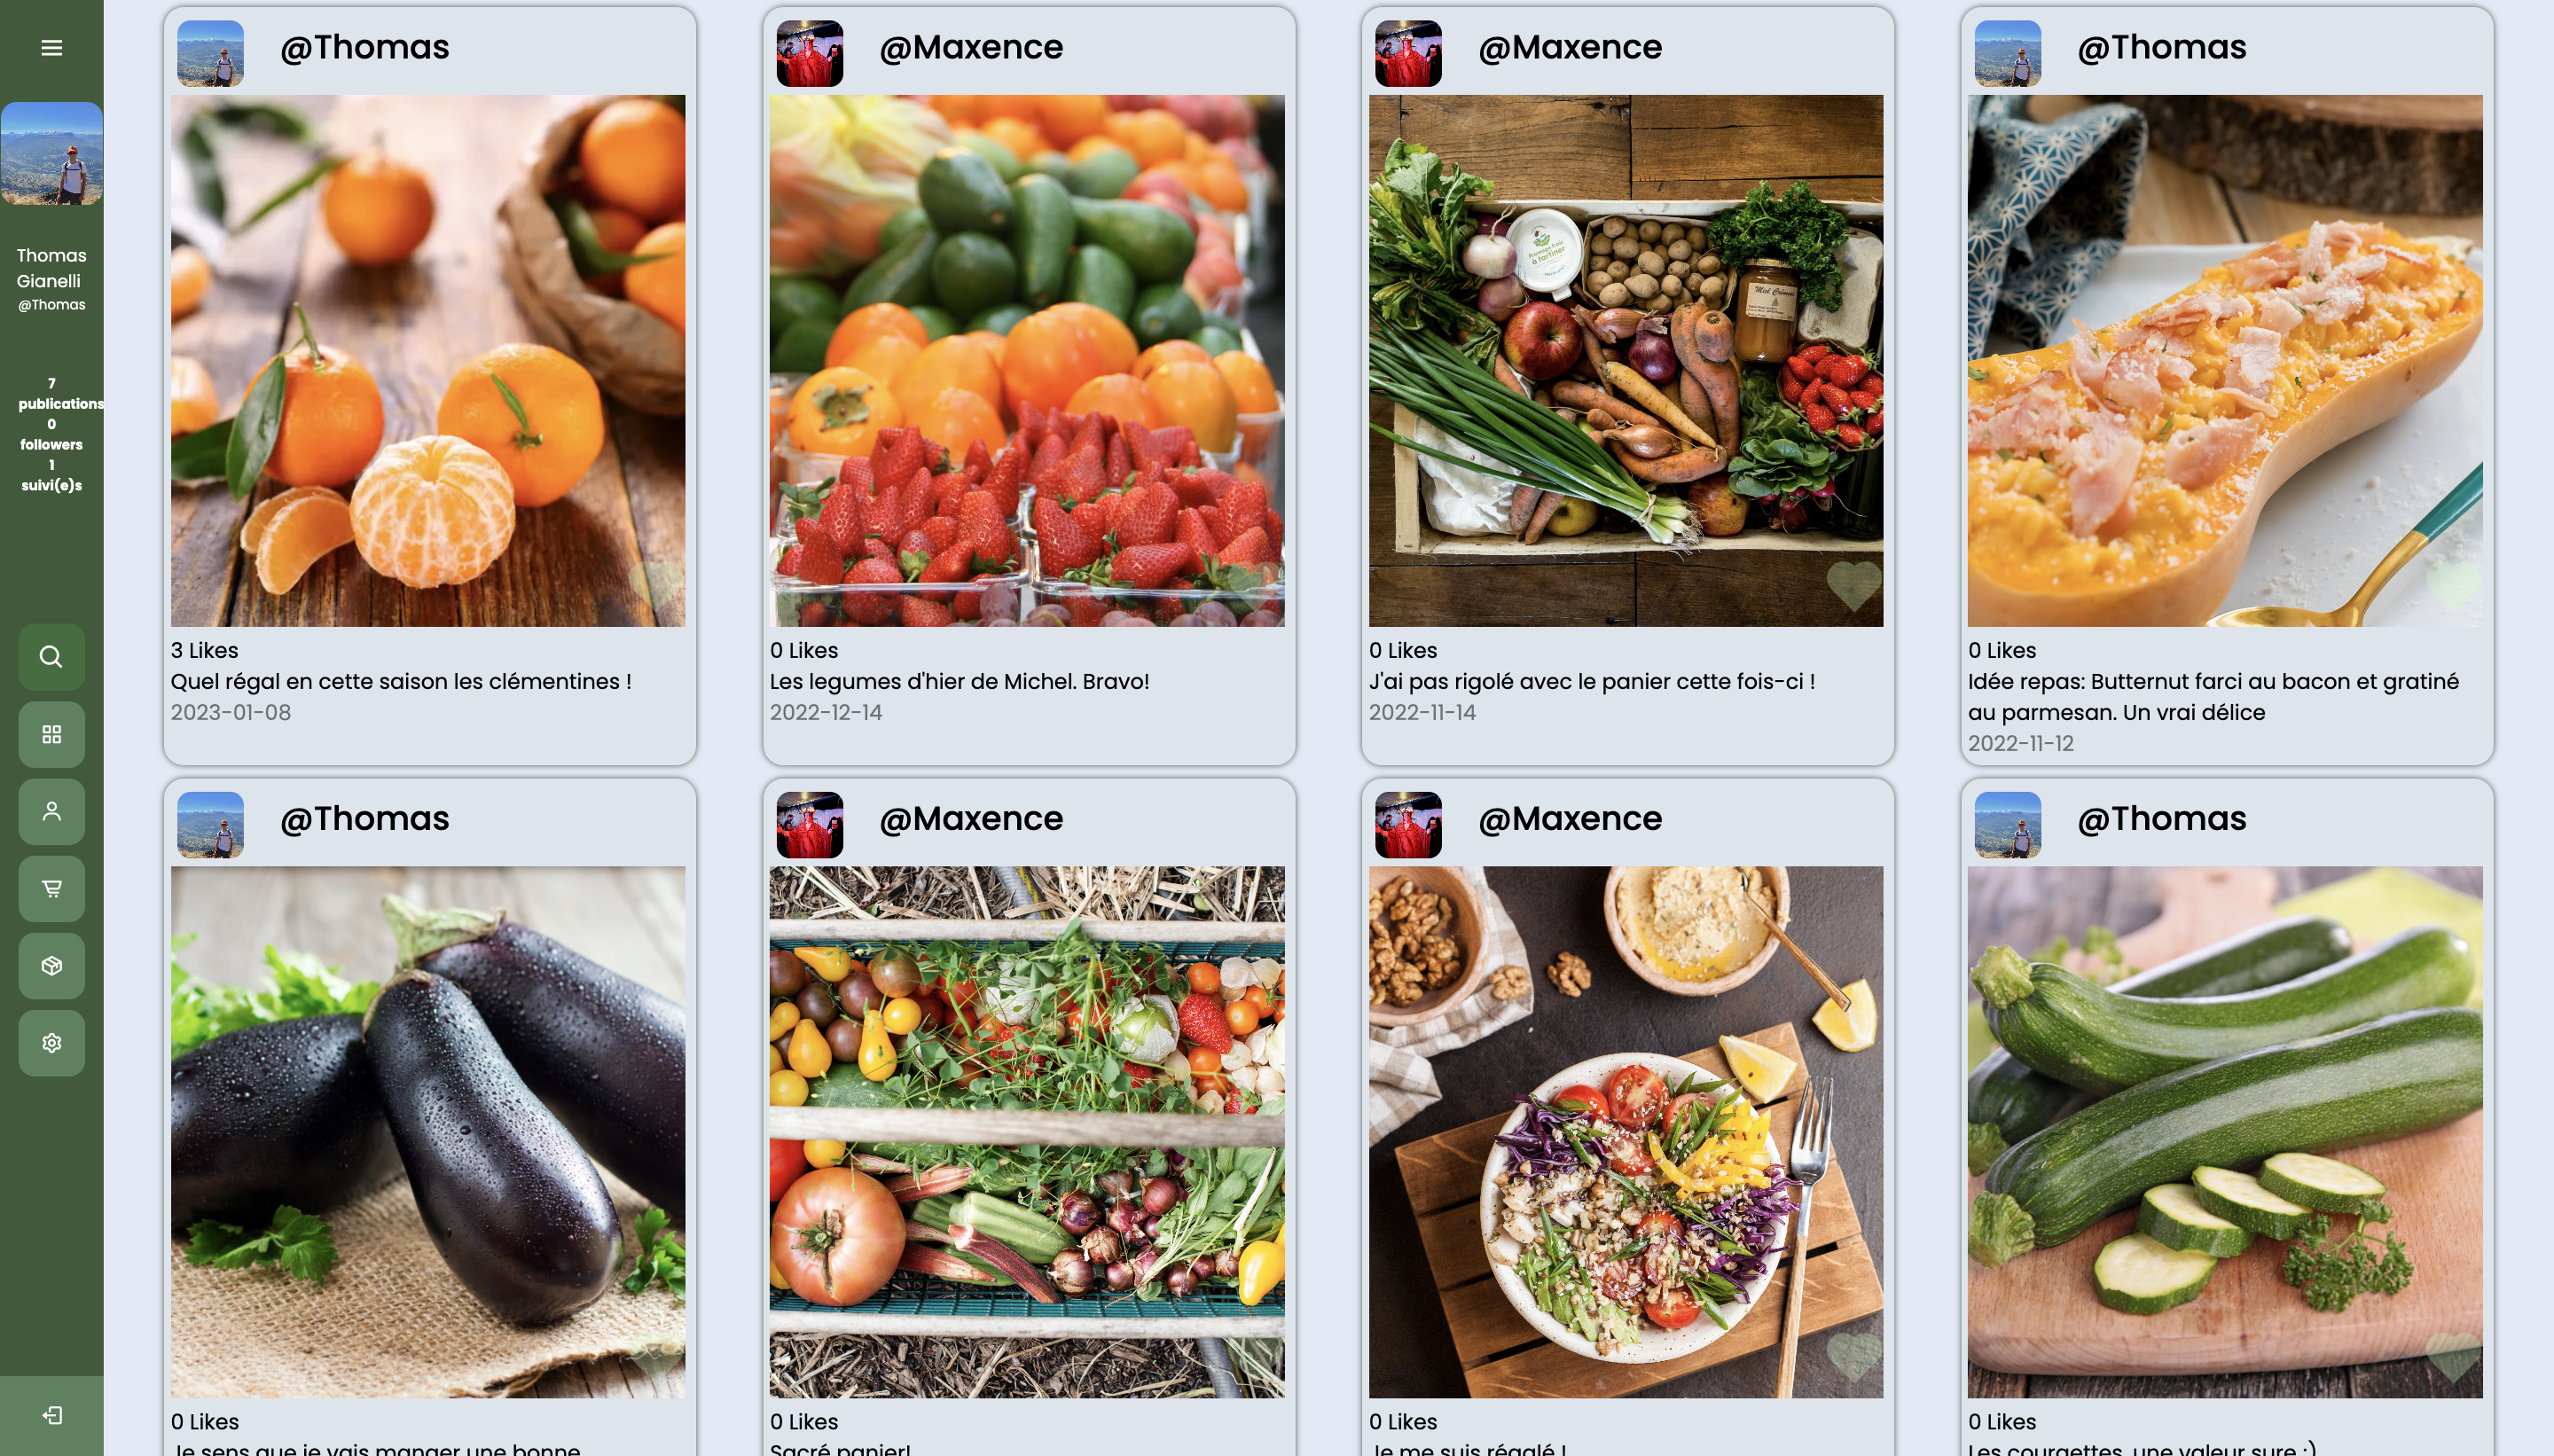
\includegraphics[scale=0.33]{ScreenPublications.png}
    \caption{Rendu de la page \texttt{publications.html}}
\end{figure}

Voici donc un exemple de rendu de la page \texttt{publications.html}.

\subsubsection{potag\_vente.py}
Nous avons regroupé dans ce module les fonctions liées à la vente :

\begin{itemize} 
\item \texttt{ventes()} pour voir les legumes vendus par les producteurs
\item \texttt{addventes()} pour ajouter des legumes
\item \texttt{lockers()} pour voir l'emplacement des lockers
\item \texttt{achats()} pour voir ses achats
\end{itemize} 

Les fonctions ventes et addventes fonctionnent sur le même principe que publications et addpublications, à la différence que les likes deviennent des achats. La fonction achats fonctionne sur le même principe que followers.

Lors d'un achat, l'objet n'est plus visible pour les autres, l'acheteur et le vendeur sont ajoutés en file d'attente et le nombre d'achats augmente.

Un des avantages de flask est l'utilisation de boucle dans l'html afin d'afficher un nombre de publications ou d'achats qui depend de la base de donnée.

\begin{lstlisting}[language=html, caption={Boucle dans le code html de \texttt{achats.html}}]

    <div class="ligne">
        <div class="photo">
            <img src="{{achat[3]}}">
        </div>
        <div class="username">
            <a href="/visitprofile{{achat[1]}}">{{achat[1]}}</a>
        </div>
        <div class="nb_publications">
            description: {{achat[2]}}
        </div>
        <div>
        <form action="/achats" method="POST">
            <div class="annulation">
            <input type="hidden" name="idpost" value={{achat[0]}} >
            <button type='submit'>Annuler</button>
            </div>
        </form>
        </div>
    </div>

\end{lstlisting}
Ici le bloc est répété pour chacun des éléments de la liste \texttt{achats}. On peut aussi appeler des variables avec \{\{variable\}\}.

\begin{figure}[h]
    \centering
    \includegraphics[scale=0.35]{ScreenAchats.png}
    \caption{Exemple de rendu de la page \texttt{achats.html}}
\end{figure}

\subsubsection{potag\_preferences.py}

Enfin, dans ce module nous avons regroupé toutes les fonctions relatives aux paramètres de l'utilisateurs:

\begin{itemize}
    \item \texttt{parametres()} pour voir les différents paramètres
    \item \texttt{profile\_picture()} pour changer sa photo de profil   
    \item \texttt{changeadress()} pour changer son adresse
    \item \texttt{changepassword()} pour changer son mot de passe
    \item \texttt{deleteaccount()} pour supprimer son compte
\end{itemize}
\vspace{0.4cm}

Nous allons cette fois-ci un petit peu détailler la fonction \texttt{profile\_picture()} car nous n'avons pas encore présenté la façon de charger une image sur notre application.

\begin{lstlisting}[language=python, caption={Fonction Python \texttt{profile\_picture.html}}]
def profile_picture():
    active=recup_infos()
    if not active:
        return redirect('/')
    if request.method == "POST":
        file = request.files['file']
        filename=file.filename # On note le nom du fichier envoyé par l'utilisateur
        if filename=='': # Si le nom est vide c'est qu'aucun fichier n'a été envoyé
            error="Veuillez sélectionner une image"
            return render_template("profilepicture.html", error=error)
        file.save(UPLOAD_FOLDER+ 'profils/' + 'pp' + session["name"] + '.png') # On enregistre le fichier en le renommant
        db = sqlite3.connect(DATABASE)
        cursor= db.cursor()
        chemin= UPLOAD_FOLDER + 'profils/' + 'pp' +session["name"]+'.png'
        if session["compte"]=='acheteur':
            cursor.execute("UPDATE acheteur SET profile = ? WHERE id_acheteur = ?", (chemin, session["name"]))
        else:
            cursor.execute("UPDATE producteur SET profile = ? WHERE id_producteur = ?", (chemin, session["name"]))
        db.commit() # On insére dans la base de données le chemin du fichier
        db.close()
        return redirect("/profil")
    info=session["infos_perso"]
    return render_template("profilepicture.html",compte=info)
\end{lstlisting}

Comme presque toutes les fonctions de notre application, on commence par vérifier si un utilisateur est connecté. Dans ce cas, on recupère des infos relatives à son profil.

Si une requête de type \texttt{POST} est effectuée sur la page, on récupère le fichier envoyé par l'utilisateur et le nom du fichier. Si ce nom est la chaîne vide, c'est qu'aucun fichier n'a en réalité été envoyé par l'utilisateur. Dans ce cas on l'invite à envoyer de nouveau un fichier. Dans le cas contraire, c'est que l'utilisateur a envoyer un fichier au format \texttt{.jpeg} ou \texttt{.png} car seules ces formats sont acceptés par notre code \texttt{html}. On enregistre alors le fichier dans un dossier prédéfini en prenant soin de le renommer selon un schéma bien précis. Une fois le fichier enregistré, on insère dans la base de données le chemin menant à l'image, afin de pouvoir la récupérer facilement.

\begin{figure}[h]
    \centering
    \includegraphics[scale=0.4]{ScreenPhotoProfil.png}
    \caption{Page de changement de la photo de profil}
\end{figure}

\subsection{Algorithmes}

Dans notre projet PotaG, lors de l'achat du produit d'un producteur par un acheteur, un casier doit leur être attribué afin de procéder à l'échange. Il ne faut pas que le casier attribué soit trop loin pour les deux personnes concernées. Aussi, il faudrait essayer d'harmoniser les distances entre chaque partie et le casier, et cela pour plusieurs transactions à la fois. C'est pourquoi nous avons mis en place une liste d'attente qui est traitée par l'algorithme une fois remplie. L’algorithme en question doit donner la meilleure suite de casiers pour les couples de la liste d'attente.

\subsubsection{Notion d'ordre}
Un couple est constitué de l'id d'un acheteur et d'un vendeur: (Thomas, Michel). Nous allons d'abord récupérer la distance pour l'acheteur et pour le vendeur à chaque casiers. Nous aurons donc une liste avec des tuples contenant: la distance acheteur, la distance vendeur, le numero de casier: $$[(1, 3, 0),(2, 3, 1),...,(a_1, a_2, a_3)]$$ on répète cela pour chacun des couples de la liste d'attente. Il nous faut ensuite trier ces listes. Mais comment juger de l'ordre pour des tuples (en sachant que le numéro de casier n'entre pas en compte). L'ordre lexicographique (ordre du premier élément puis du deuxième) n'est pas judicieux car il pénalise le vendeur. Après quelques tests, un ordre semble intéressant: $\sqrt{{a_1}^2+{a_2}^2}$.

En posant
\begin{itemize}
\item $a=(a_1, a_2) $
\item $b=(b_1, b_2)$ 
\item $\sqrt{{a_1}^2+{a_2}^2}<\sqrt{{b_1}^2+{b_2}^2}\implies a <b $
\end{itemize}
\vspace{0.4cm}

On obtient un ordre qui favorise les petites distances mais aussi les petits écarts entre $a_1$ et $a_2$.

\subsubsection{Tri Fusion}
Nous avons besoin de trier les listes car nous voulons savoir quel casier est le meilleur pour un couple acheteur-vendeur donné. Si le premier casier n'est pas disponible, on choisira le suivant et ainsi de suite.
Parmi les tris que l'on connait, le tri fusion se place comme un bon candidat: il est simple à mettre en oeuvre, présente une complexité optimale en $n\times\log(n)$ pour une liste de taille n et fonctionne parfaitement avec des listes.
Il est basé sur le principe algorithmique diviser pour régner. Le tri fusion fonctionne de manière récursive: pour trier une liste A, on trie la moitié droite et la moitié gauche puis on les fusionne. Un tableau à un seul élément est déjà trié.

\begin{lstlisting}[language=python, caption={Appel recursif}]
def tri_fusion(tableau):
    if  len(tableau) <= 1: 
        return tableau
    pivot = len(tableau)//2
    gauche = tri_fusion(tableau[:pivot])
    droite = tri_fusion(tableau[pivot:])
    return fusion(gauche,droite)
\end{lstlisting}

Pour fusionner deux tableaux triés, on parcourt les deux tableaux parallèlement en ajoutant dans le tableau final le plus petit des deux éléments.
C'est donc ici l'on implémente l'ordre choisi. 

\begin{lstlisting}[language=python, caption={Fusion de deux tableaux triés selon l'ordre choisi précédemment}]
def fusion(tableau1,tableau2):
        indice_tableau1 = 0
        indice_tableau2 = 0    
        taille_tableau1 = len(tableau1)
        taille_tableau2 = len(tableau2)
        tableau_fusionne = []
        while indice_tableau1<taille_tableau1 and indice_tableau2<taille_tableau2:
            val1 = sqrt(tableau1[indice_tableau1][0]**2 + tableau1[indice_tableau1][1]**2)
            val2 = sqrt(tableau2[indice_tableau2][0]**2 + tableau2[indice_tableau2][1]**2)
            if val1 < val2:
                tableau_fusionne.append(tableau1[indice_tableau1])
                indice_tableau1 += 1
            else:
                tableau_fusionne.append(tableau2[indice_tableau2])
                indice_tableau2 += 1
        while indice_tableau1<taille_tableau1:
            tableau_fusionne.append(tableau1[indice_tableau1])
            indice_tableau1+=1
        while indice_tableau2<taille_tableau2:
            tableau_fusionne.append(tableau2[indice_tableau2])
            indice_tableau2+=1
        return tableau_fusionne
\end{lstlisting}

Dans notre projet l'appel est fait sur des listes de taille $n=$ "le nombre de casier". Dans notre exemple sur Nancy il y a 18 casiers donc $n=18$. 

\subsubsection{Backtracking}
Il nous faut maintenant trouver la meilleure suite de casiers afin que chacun des couples se voit attribué le casier avec le plus faible score ($\sqrt{{distance_{acheteur}}^2+{distance_{vendeur}}^2}$) possible.
L'algorithme est le suivant pour 3 couples, deux casier, un d'une place et l'autre de deux places:
\begin{itemize}
    \item On suppose que l'on a pour chaque couple la liste des distances aux casiers triée. Le troisième élément étant le numéro du casier (0 ou 1 dans notre exemple).
\end{itemize}

\begin{center}
\hspace{-1.75cm}\begin{tabular}{ c c| c| c }
    & Pierre-Paul & Théo-Antoine & Thomas-Michel \\
    Choix 0 & (1,4,0) & (2,4,1) & (1,3,0) \\
    Choix 1 &  (2,8,1) & (3,5,0) & (2,4,1) \\
 \end{tabular}
\end{center}

\begin{itemize}
    \item On choisit d'abord le premier choix pour chacun.
\end{itemize}

\begin{center}
\begin{tabular}{ c| c| c }
    Pierre-Paul & Théo-Antoine & Thomas-Michel \\
  \textbf{(1,4,0)} & \textbf{(2,4,1)} & \textbf{(1,3,0)} \\
 (2,8,1) & (3,5,0) & (2,4,1) \\
 \end{tabular}
\end{center}

\begin{itemize}
    \item On parcourt ensuite les couples. On vérifie qu'il y a de la disponibilité dans le casier voulu. Si c'est le cas on passe au couple suivant. Sinon on regarde si un autre couple avant celui-ci n'a pas déjà pris ce casier. Si c'est le cas, c'est celui qui a le meilleur score qui le garde, et l'autre passe à son deuxième choix. Sinon, c'est qu'il n'y a plus de place, alors le couple passe à son deuxieme choix.  On valide le choix de Pierre-Paul puis celui de Théo-Antoine. Le choix de Thomas-Michel ne peut pas être  validé car la seule place du casier 0 est déjà attribuée à Pierre-Paul. Comme on a $\sqrt{1+3^2}<\sqrt{1+4^2}$, c'est à Thomas-Michel que le casier est attribué. Pierre-Paul passe donc à son deuxième choix et on relance l'algorithme
\end{itemize}

\begin{center}
\begin{tabular}{ c| c| c }
   Pierre-Paul & Théo-Antoine & Thomas-Michel \\
   (1,4,0) & \textbf{(2,4,1)} & \textbf{(1,3,0)} \\
   \textbf{(2,8,1)} & (3,5,0) & (2,4,1) \\
 \end{tabular}
\end{center}

\begin{itemize}
    \item L'algorithme se finit quand on a parcouru toute liste puisque dans ce cas c'est que les choix sont tous valides. Dans notre exemple on retourne donc 1,1,0
\end{itemize}

\begin{center}
\begin{tabular}{ c| c| c }
   Pierre-Paul & Théo-Antoine & Thomas-Michel \\
   1 & 1 & 0 \\
 \end{tabular}
\end{center}

Pour le code python on a besoin d'une fonction \texttt{premier\_meme} pour trouver le premier couple ayant le casier voulu.

\begin{lstlisting}[language=python, caption={Fonction python \texttt{premier\_meme}}]
def premier_meme(liste,i):
        for j in range(len(liste)):
            if liste[i]==liste[j] and j!=i:
                return True,j
        return False,0
\end{lstlisting}

Cet algorithme renvoit True et l'indice de la première apparition si il y en a une, False et 0 sinon.
Ensuite il faut une fonction récursive qui applique le parcours de la liste jusqu'à pouvoir la parcourir en entier.

\begin{lstlisting}[language=python, caption={Implémentation de l'algorithme récursif}]
   def rec_aux(liste,dispo,choix,fin):
        dispo_cop = dispo[:]
        for couple in range(len(liste)):
            testeur = premier_meme(liste,couple) # Autre couple qui a le meme casier
            if dispo_cop[fin[couple]]>0: #Il reste de la place,il garde ce casier
                dispo_cop[fin[couple]]-=1
            elif testeur[0]: #Sinon, le plus faible score garde le casier
                ach1 = liste[couple][choix[couple]][0]
                vend1 = liste[couple][choix[couple]][1]
                ach2 = liste[testeur[1]][choix[testeur[1]]][0]
                vend2 = liste[testeur[1]][choix[testeur[1]]][1]
                val1 = sqrt( ach1**2 + vend1**2)
                val2 = sqrt( ach2**2 + vend2**2)
                if val1>val2: # On teste le score
                    choix[couple]+=1
                    fin[couple] = liste[couple][choix[couple]][2]
                else: 
                    choix[testeur[1]]+=1
                    fin[testeur[1]] = liste[testeur[1]][choix[testeur[1]]][2]
                return rec_aux(liste,dispo,choix,fin) 
            else: #Plus de place et personne n'a le casier: passe au choix suivant
                choix[couple]+=1
                fin[couple] = liste[couple][choix[couple]][2]
                return rec_aux(liste,dispo,choix,fin)
        return fin #On a finit une boucle donc l'attribution des casiers est valide 
\end{lstlisting}

On commence l'algorithme avec le premier choix de chacun des couples. L'appel à la fonction recursive se fait donc :

\begin{lstlisting}[language=python, caption={Implémentation de l'algorithme récursif}]
def backtrack_meilleur(liste,dispo):
    choix_numero = [0 for i in range(len(liste))]
    casiers = [liste[i][0][2] for i in range(len(liste))]
    return rec_aux(liste,dispo,choix_numero,casiers)
\end{lstlisting}




\section{Tests et Performances}

\subsection{Tri Fusion}
\subsubsection{Tests}
Pour tester l’algorithme, il faut dans un premier temps générer des listes de couples de réels. Pour cela, on utilise la fonction \texttt{uniform} du module \texttt{random}. Elle nous permet de générer un réel entre 0 et $x$ aléatoirement, avec $x$ la borne max choisie. On construit donc la fonction \texttt{gen\_liste\_aleat} qui va générer des listes de couples de réels aléatoires.
\vspace{0.4cm}

\begin{lstlisting}[language=Python, caption={ Fonction \texttt{gen\_liste\_aleat.py} }]
def gen_liste_aleat(n,x):
    #liste (taille n) de couple de réel aléatoire entre 0 et x m
    liste = [[random.uniform(0,x),random.uniform(0,x)] for i in range(n)]
    return liste 
\end{lstlisting}
\vspace{0.4cm}

Dans un deuxième temps, il faut vérifier que le tri fonctionne. Pour ça, on utilise la fonction \texttt{sorted} de python, avec key=norme, ce qui donne le même résultat que notre algorithme de tri.
\vspace{0.4cm}

On va procéder à deux tests différents :

\begin{itemize}

\item un test dans les conditions réelles de notre application : un nombre de transactions et d’adresses de casiers cohérentes ainsi que des distances qui restent locales. 

\item un test dans des conditions plus générales de l’algorithme.
\end{itemize}
\vspace{0.4cm}
Dans le cas réel, on choisit 16 adresses de casiers et 50 personnes soit 800 couples à trier. Les distances restent inférieures à 10 km. 
\vspace{0.4cm}


\begin{lstlisting}[language=Python, caption={ Fichier de test : \texttt{test\_1.py} }]
from test_algo import *
"""
test de tri fusion dans le cas reel
"""
t = [None for x in range(800)]
temps_exec = [None for x in range(800)]
correction = True
 
for i in range(0,800):
   # generation de la liste aleatoire de taille i, de reel entre 0 et 10k
   t[i] = gen_liste_aleat(i,10000)
 
   # teste de correction
   temp_correction =(tri(t[i])==trie_fusion_liste_distance(t[i]))
   if temp_correction==False:
       correction = False
 
#correction de l'algo
def test_cas_reel():
   assert correction
\end{lstlisting}

   
Le code \texttt{test\_1.py} permet de réaliser le test dans le cas réel. La correction est la variable importante : elle reste à vrai si aucune faute n’est commise, elle passe à faux si au moins un test est faux. La fonction \texttt{test\_cas\_reel} est invoqué par \texttt{pytest} avec la commande : \texttt{pytest -v test\_1.py}

\newpage %provisoire pour mise en page

\begin{figure}[h]
     \centering
     \includegraphics[scale=0.7]{pytest_test_1.png}
     \caption{Invoquation de \texttt{pytest} pour tester le tri fusion}
 \end{figure}


Dans le cas général, on va aller jusqu'à des listes de 20 000 éléments (chaque liste générée a 10 éléments de plus que la précédente) et des distances de l'ordre de la centaine de kilomètres.
De même on teste avec pytest (fichier \texttt{test\_2.py}), le test dure 1 minute 30 environ et nous donne un résultat positif.

\subsubsection{Performance}
On récupère les temps d'exécution dans le cas réel et dans le cas général.
On obtient : 
\begin{figure}[h]
     \centering
     \includegraphics[scale=0.6]{tri_fusio_temps_reel.png}
     \centering
     \includegraphics[scale=0.6]{tri_cas_general.png}
     \caption{Temps d'exécution en fonction de la taille de la liste}
\end{figure}

Les temps d’exécutions sont cohérents avec la complexité du tri fusion en $n \times \log(n)$. Cette complexité est optimale et conviendra pour une application à plus grande échelle. Par contre, il faut noter que la complexité spatiale est de l'ordre de $n$. Cela ne posera pas problème puisque la taille des listes n'augmentera pas, le nombre de point de vente dans une ville etant limité.

\subsection{Backtracking}
\subsubsection{Tests}
Nous allons utiliser une propriété intéressante : si pour chaque point de vente, il y a plus de casiers disponible que de transactions, chaque couple se voit attribuer le casier le plus proche. Il est important que l'algorithme fonctionne correctement dans ce cas particulier.
\vspace{0.4cm}


Afin de mener au mieux nos tests, nous avons modifié la fonction \texttt{traite\_liste} pour obtenir la distance au casier le plus proche et la distance au casier attribuée par l'algorithme. Également il nous fallait pouvoir accéder aux adresses et disponibilités des casiers ainsi qu'aux adresses des acheteur et vendeur sans passer par une base de données. La fonction modifiée est la suivante :
\vspace{1.2cm}

\begin{lstlisting}[language=Python, caption={ Fonction \texttt{traite\_file} modifiée pour les tests }]
def traite_file_test_distance(file,dispo,liste_casiers):
    distance_par_couple = []
    distance_min=0
    for couple in file:
        liste_distance=[]
        for i in range(len(liste_casiers)):
            casier = liste_casiers[i]
            prem = get_distance(couple[0],casier)
            deux = get_distance(couple[1],casier)
            liste_distance.append([prem,deux,i])
        liste_distance = trie_fusion_liste_distance(liste_distance)
        distance_min+=liste_distance[0][0]+liste_distance[0][1] #somme des plus petites distances parcouru
        distance_par_couple.append(liste_distance)
    casiers=backtrack_meilleur(distance_par_couple,dispo)
    distance_final = 0
    for i in range(len(casiers)):
        for e in distance_par_couple[i]:#liste des distances pour le couple e
            if e[2]==casiers[i]:
                distance_final+= e[0]+e[1]#distance choisi par l'algo de backtracking
    return distance_min,distance_final
\end{lstlisting}
\vspace{0.4cm}
La fonction renvoie \texttt{distance\_min} et \texttt{distance\_final} :\begin{itemize}
    \item \texttt{distance\_final} correspond à la somme des distances parcourues par chaque couple acheteur/vendeur
    \item \texttt{distance\_min} correspond à la somme des distances minimales pour chaque couple.
\end{itemize}{}

Pour le premier test, on va vérifier que ces deux distances sont égales.
\vspace{0.4cm}

Pour effectuer les tests de la fonction il nous faut des adresses pour les acheteurs, les vendeurs, mais aussi pour les casiers. Pour les créer, nous avons derminé les coordonnées gps du centre de Nancy et choisi des points gps au hasard dans un périmètre donné :

\begin{lstlisting}[language=Python, caption={création de points gps autour du centre de Nancy }]
lat = 48.692054 #latitude d'un point central de Nancy
lon = 6.184417 #longitude d'un point central de Nancy
perimetre = 0.05 #distance des utilisateurs au point gps {lat,lon} 
point = [lat+perimetre*(2*(random.random()-1)),lon+perimetre*(2*(random.random()-1))]
\end{lstlisting}

Cette méthode pose problème car elle peut générer des points non-accessible par un itinéraire Google map : il faut donc vérifier que le point créé permet de déterminer un itinéraire. On fait donc appel à \texttt{get\_distance} en levant une erreur en cas d'échec. En prévision de tous les tests on génère 1000 points gps, stockés dans le fichier \texttt{coord\_gps\_nancy.txt}. Ils sont accessibles en utilisant la fonction \texttt{get\_coord\_gps}.
\vspace{0.4cm}

On peut désormais utiliser ces points gps pour tester une première fois la fonction sur le cas particulier décrit plus haut. On définit le nombre de transactions à 10, la limite pour la file d'attente de l'algorithme, et on incrémente le nombre de casiers tout en s'assurant que chaque adresse de casier a plus de disponibilités que de transactions.
Ce test est effectué dans le fichier\texttt{ test\_3.py} par \texttt{pytest} et prend 150 secondes environ.
\vspace{0.4cm}

Pour aller plus loin dans les tests, on va comparer la \texttt{distance\_final} et la \texttt{distance\_min} pour vérifier que notre algorithme choisit des solutions optimales :
On va pouvoir mesurer l'écart à la distance minimal pour chaque couple :


\begin{lstlisting}[language=Python, caption={\texttt{test\_4.py} permet de générer les courbes de \texttt{distance\_final} et \texttt{distance\_min} }]
def delta_distance(k):
    #k est le nombre de delta différent
    distances_finales=[]
    distances_min=[]
    gps_data = get_coord_gps()
    for l in range(k):
        casier =[random.choice(gps_data) for i in range(5)] #les adresses des casiers
        couple =[[random.choice(gps_data),random.choice(gps_data)] for i in range(10)] #un couple = une transacton acheteur vendeur, 10 transactions
        dispo = [2 for i in range(5)]
        temp_test = traite_file_test_distance(couple,dispo,casier)#temp test corr
        distances_finales.append(temp_test[1])
        distances_min.append(temp_test[0])
    return  distances_finales,distances_min
\end{lstlisting}

Le code est similaire à celui de \texttt{test\_3.py}, mais on teste pour 10 transactions et 5 casiers repartis sur 2 emplacements à chaque fois, et ce $k$ fois. Chaque itération prend en moyenne 1 minute, ce qui est tout à fait acceptable pour notre application puisque cette fonction à pour objectif d'être lancé en fond sans gêner les utilisateurs. On obtient les écarts de distance suivant :


\begin{figure}[h]
     \centering
     \includegraphics[scale=0.6]{test4_graph.png}
     \caption{\texttt{distance\_final} et \texttt{distance\_min} }
\end{figure}

Les distances sont un peu en dessous de 10 km, ce qui est à la limite des zones ciblées par notre application, et les casiers ne sont pas placés de manière stratégique, ce qui explique les grandes distances.
\vspace{0.4cm}


\subsubsection{Performance}
Nous allons observer le comportement de l’algorithme en fonction du nombre de casiers et de personnes puis comparer la complexité obtenue avec la théorique après l'avoir définie.
\vspace{0.4cm}

Dans un premier temps, afin de mesurer et d'évaluer le temps d'exécution pour un nombre de casiers croissant nous allons utiliser la fonction \texttt{process\_time} du module \texttt{time}. Elle va nous permettre d'obtenir le temps qu'a passé le processeur sur notre algorithme :
\vspace{0.4cm}

\begin{lstlisting}[language=Python, caption={Mesure du temps d'exécution de \texttt{traite\_file\_test\_distance}}]
    start = time.process_time()
    temp_test = traite_file_test_distance(couple,dispo,casier)
    end = time.process_time()-start
\end{lstlisting}
\newpage
Le code pour la mesure du temps se trouve dans \texttt{test\_5.py}. Il donne :

\begin{figure}[h]
     \centering
     \includegraphics[scale=0.6]{graph_test5_process_time.png}
     \caption{Temps d'éxecution processeur du backtracking en fonction du nombre de casiers} 
\end{figure}

Cependant, le temps total d'exécution, en comptant le temps d'attente à l'API peut être mesuré à l'aide de \texttt{perf\_counter} du module \texttt{time} :

\begin{figure}[h]
\centering
\includegraphics[scale=0.6]{graph_test5_perf_counter.png}
\caption{temps d'exécution total du backtracking en fonction du nombre de casiers} 
\end{figure}
La partie lente de l'algorithme provient de l'API Google Maps, qui multiplie par 10 le temps d'exécution.
\newpage
On peut aussi mesurer le temps moyen pour des valeurs proches de notre utilisation, soit 9 casiers et 10 transactions :
\begin{figure}[h]
     \centering
     \includegraphics[scale=0.6]{graph_test6.png}
     \caption{temps d'exécution total du backtracking dans le cas de notre application} 
\end{figure}

Il nous faut ensuite déterminer la complexité théorique de notre algorithme de backtracking afin de la comparer à celle observée. Dans le meilleur des cas on parcourt une première fois la liste et tous les casiers choisis sont valides, la complexité est de $n$.
Dans le pire des cas, à chaque passage le choix du dernier couple n'est pas valide. On rappelle donc la fonction juste avant la fin du parcours de la liste. On suppose aussi que toutes les personnes obtiennent leur dernier choix, ce qui donne $n\times n \times nombre\_de\_casiers$, donc de l'ordre de $n^2$. Aussi l'appel à \texttt{premier\_meme} est de complexité $n$ dans le pire des cas avec le parcours de la liste. Au final la fonction est de complexité $n^3$ dans le pire des cas.

\section{Gestion de projet}

\subsection{Cahier des charges fonctionnel}

Les différentes parties de ce cahier des charges:
\begin{itemize} 
\item Groupe d’expression du besoin
\item Historique des modifications et révisions de ce document
\item Résultats et changements attendus
\item Parties prenantes
\item Contraintes de planning
\end{itemize}

\subsubsection{Auteurs de ce cahier des charges / groupe d’expression du besoin}
\begin{center}
	\begin{tabular}{|l|l|}
	\hline
		\textbf{Nom / email}	& \textbf{Qualité / rôle}\\
		\hline
Maxence BEKHEDDA / maxence.bekhedda@telecomnancy.eu&
Membre de l’équipe projet\\
\hline
Léo GERMAIN / leo.germain@telecomnancy.eu&
Membre de l’équipe projet\\
\hline
Thomas GIANELLI / thomas.gianelli@telecomnancy.eu&
Membre de l’équipe projet\\
\hline
Théo WALTER / theo.walter@telecomnancy.eu&
Membre de l’équipe projet\\
\hline
\makecell[l]{
Olivier FESTOR / olivier.festor@telecomnancy.eu\\
Anne-Claire HEURTEL / anne-claire@telecomnancy.eu\\
Gérald OSTER / gerald.oster@telecomnancy.eu}&
Commanditaires\\
\hline
	\end{tabular}
\end{center}






\subsubsection{Historique des modifications et révisions de ce document}
\begin{center}
	\begin{tabular}{|c|c|c|}
	\hline
	\textbf{n° de version} &	\textbf{Date}	&\textbf{Description et circonstances de la modification}\\
	\hline
    V1&	19/10/2022&	1ère version du cahier des charges en vue de la 1ère soutenance\\
    \hline
    V2 & 10/11/2022&Utilisation concrète des outils de gestion de projet\\
    \hline
	\end{tabular}
\end{center}


\subsubsection{Résultats et changements attendus}
	Livrables : 
	\begin{itemize}
		\item 	\color{red} Premier rapport \color{black}, écrit en LaTex, en trois sections : l’état de l’art, le concept et la gestion de projet.
		\item	\color{red} Présentation pour la première soutenance \color{black} sur l’état de l’art, le concept et la gestion de projet.
		\item	\color{red} Second rapport \color{black} avec une section pour l’implémentation de la base de données, du serveur web et des algorithmes de traitement, une section consacrée aux tests et aux performances puis une dernière section pour la gestion de projet.
		\item   \color{red} Présentation pour la seconde soutenance \color{black} sur l’application et la gestion de projet puis démonstration des fonctions.
	\end{itemize}
	
\subsubsection{Parties prenantes}
L'objectif de cette partie est de recenser exhaustivement tous les acteurs concernés par le projet et ses conséquences. 
\vspace{0.2cm}

\noindent Commanditaires: 
\begin{itemize}
	\item 
	initiateurs du projet : Olivier FESTOR, Anne-Claire HEURTEL, Gérald OSTER 
	\end{itemize}
	
\vspace{0.2cm}

\noindent Équipe de réalisation:
\begin{itemize}
	\item Maxence BEKHEDDA
	\item Léo GERMAIN
	\item Thomas GIANELLI
	\item Théo WALTER
\end{itemize}

\vspace{0.2cm}

\noindent Autres parties prenantes :
\begin{itemize}
	\item utilisateur finaux : particulier souhaitant vendre ses fruits et légumes en circuit-court, toute personne souhaitant acheter des fruits et légumes produit par des particuliers à proximité.
		\item	soutiens et opposants au projet : les autres groupes formés d’élèves de 1A créant des applications web répondant au même besoin
		\item	personnes-ressources et experts : Christophe BOUTHIER, Olivier FESTOR, Anne-Claire HEURTEL, Gérald OSTER 
\end{itemize}


\subsubsection{Contraintes de planning}
\begin{itemize}
	\item 	1er rapport : 20/10/2022 à 18h
		\item	1ère soutenance : 22/10/2022 à 9h
		\item	Date de rendu du projet : 11/01/2023 à 12h
		\item	Date de soutenance : 19/01/2023 à 16h
\end{itemize}


\subsection{To-Do List}
\subsubsection{To-Do List en vue de la première soutenance}

\rotatebox{90}{
	\begin{tabular}{|c|c|c|c|c|c|c|c|}
\hline
	\textbf{Tâches} & 
		\makecell[c]{\textbf{Priorité}\\
		\textbf{(0-4)} \\}& 
		\makecell[c]{\textbf{Date} \\\textbf{de} \\\textbf{début} }& 
		\makecell[c]{\textbf{Date} \\\textbf{de}\\ \textbf{fin}} &
		\makecell[c]{\textbf{Charge}\\ \textbf{de}\\ \textbf{travail}} & 
		\textbf{Livrables} & 
		\textbf{Progrès} & 
		\makecell[c]{\textbf{Dernière} \\\textbf{mise à}\\ \textbf{jour}}\\
		\hline
		État de l'art&
		4&
		10/10/22&
		18/10/22&
		8h&
		\makecell[c]{
		Chercher et relever quelques exemples\\ d’applications web de vente de fruits et\\ légumes en circuit court existantes afin \\de les mettre en perspective avec notre \\application}&
		100\%&
		17/10/22\\
		\hline
		\makecell[c]{Gérer la gestion\\ du projet}&
		2&
		10/10/22&
		18/10/22&
		6h&
		\makecell[c]{Rédiger des comptes-rendus pour chaque\\ réunion. Définir la démarche avec une \\to-do list et un cahier des charges.}&
		100\%&
		17/10/22\\
		\hline
		\makecell[c]{Expliquer le concept\\ de l'application et \\ son aspect innovant}&
		2&
		14/10/22&
		18/10/22&
		2h&
		\makecell[c]{Expliquer avec détails le concept de \\l’application. Puis, à partir de l’état de \\l’art, énoncer ses caractéristiques \\innovantes.}&
		100\%&
		17/10/22\\
		\hline
		Rédiger le rapport&
		2&
		16/10/22&
		18/10/22&
		8h&
		\makecell[c]{Rédiger un rapport détaillé reprenant \\tous les points majeurs attendus de \\notre démarche : \\
\hspace*{-1cm}-\;	L’état de l’art\\
\hspace*{0.1cm}-\;	La gestion du projet\\
\hspace*{0.8cm}-\;	L’explication du concept
}&
		80\%&
		17/10/22\\
		\hline
		\makecell[c]{Réaliser la \\ présentation}&
		2&
		16/10/22&
		18/10/22&
		4h&
		Créer un support de présentation concis&
		60\%&
		17/10/22\\
		\hline
		\makecell[c]{Préparation finale\\ en vu de la \\soutenance}&
		2&
		16/10/22&
		18/10/22&
		2h&
		\makecell[c]{Organisation des temps de parole et \\préparatifs en vue de la soutenance}&
		50\%&
		17/10/22\\
		\hline
	\end{tabular}
}	

\subsubsection{To-Do List en vue des vacances de la Toussaint}

\rotatebox{90}{
	\begin{tabular}{|c|c|c|c|c|c|c|c|}
\hline
	\textbf{Tâches} & 
		\makecell[c]{\textbf{Priorité}\\
		\textbf{(0-4)} \\}& 
		\makecell[c]{\textbf{Date} \\\textbf{de} \\\textbf{début} }& 
		\makecell[c]{\textbf{Date} \\\textbf{de}\\ \textbf{fin}} &
		\makecell[c]{\textbf{Qui?}} & 
		\textbf{Livrables} & 
		\textbf{Progrès} & 
		\makecell[c]{\textbf{Dernière} \\\textbf{mise à}\\ \textbf{jour}}\\
		\hline
		\makecell[c]{
		Création de la base \\ de donnée}&
		2&
		31/10/22&
		06/11/22&
		Léo&
		\makecell[c]{
		Création des schémas relationnels \\ et de la base de données en SQL}&
		100\%&
		06/11/22\\
		\hline
		\makecell[c]{Page de connexion}&
		2&
		31/10/22&
		06/11/22&
		Thomas&
		\makecell[c]{Page de connexion en Flask avec \\ utilisation de la base de données \\ temporaire}&
		100\%&
		06/11/22\\
		\hline
		\makecell[c]{Page d’accueil}&
		2&
		31/10/22&
		06/11/22&
		Théo&
		\makecell[c]{Page d’accueil en Flask avec utilisation \\ de la base de données temporaire}&
		100\%&
		17/10/22\\
		\hline
			\makecell[c]{Révisons des outils \\ de gestion de projet}&
		2&
		31/10/22&
		06/11/22&
		Maxence&
		\makecell[c]{Rédiger et utiliser de nouveaux outils \\ de gestion de projet tels que :   \\
\hspace*{-2.5cm}-\;Les ToDo listes\\
\hspace*{0.4cm}-\;Le cahier des charges fonctionnel\\
}&
		80\%&
		17/10/22\\
		\hline
	\end{tabular}
}	

\subsubsection{Utilisation des To-Do List}

Les To-Do List sont des outils nous permettant de nous organiser dans la répartition des tâches, de nous fixer des deadlines et d'avoir connaissance de l'avancée de chacun dans ses objectifs. 

Cependant, la plupart de ces informations sont fixées pendant les réunions et existent par conséquent déjà dans les compte-rendus qui seront présentés par la suite. Afin d'éviter la multiplication inutile d'outils de gestion de projet et de gagner du temps, nous nous sommes par la suite contentés des informations contenues dans les comptes-rendus de réunion. 

\subsection{Compte-rendus de réunion}
\subsubsection{Modèle type de compte-rendu}

\begin{center}

\begin{tabular}{|p{8.3cm}|p{8.3cm}|}
\hline

	 Motif / type de réunion: Réunion de chantier &  
	 Lieu: Telecom Nancy (1.33)\\
	 
	\hline 
	
	Présent(s) (retard/excusés/non excusés):&
	Date / heure de début:\\
	
	\makecell[lll]{
	Équipe-projet : &
 BEKHEDDA Maxence \\
& GERMAIN Léo \\
& GIANELLI Thomas \\
& WALTER Théo}&
	\makecell[l]{
10/12/2022 à 10h30\\
Durée : 40min}\\
\hline

\end{tabular}

\end{center}

\underline{Ordre du jour}

\begin{enumerate}

	\item 
		Retour sur le travail effectué par chacun depuis la dernière réunion.
\item 	Difficultés rencontrées.
\item 	Listing et répartition des tâches restantes.

\end{enumerate}

\vspace{0.5cm}

\underline{Informations échangées}
\vspace{0.2cm}

\begin{itemize}
    \item   Les objectifs fixés lors de la dernière réunion ont été accomplis sans rencontrer de difficultés particulières.
	\item 	Plusieurs fonctionnalités (notamment l'onglet "profil") réutilisent le code de l'onglet "publications". Il est donc nécessaire de le faire en priorité afin de pouvoir avancer. 
	\item 	Le style n'est pas une priorité, il vaut mieux coder quelque chose de fonctionnel permettant de débloquer de nouvelles fonctionnalités et faisant avancer le projet. On pourra s'occuper du style dans un second temps.
    \item   La date de rendu est le 6 janvier 2023. Cette date étant proche, il faut concentrer nos forces sur l'écriture code. La rédaction du rapport et la conception du support de présentation pour la soutenance viendront dans un second temps.
\end{itemize}

\vspace{0.5cm}

\underline{Remarques / Questions}
\vspace{0.2cm}

\begin{itemize}
	\item Remarque 1 : Pour nous en sortir dans cette période de "dernière ligne droite" avant le rendu du projet, cela pourrait être une bonne idée de lister les objectifs que nous souhaitons nous fixer d'ici le 6 janvier.
	\item Question 2 : Afin d'intégrer de l'algorithmique dans notre projet, nous souhaitons créer un programme permettant de calculer les casiers les plus proches de l'acheteur et du producteur qui sont disponibles. Comment mettre cela en place?
	\item Question 3 : Dans la même optique d'ajouter de l'algorithmique au projet, qu'en est-il de l'idée d'ajouter un algorithme de recommandation en fonction des récents achats et de la localisation, suggérant ainsi des publications plus probable d'être utile à l'utilisateur?

\end{itemize}

\vspace{0.5cm}
\newpage       %pour faire en sorte que Décisions soit pas décalé%
\underline{Décisions} 
\vspace{0.2cm}

\begin{itemize}
	\item  Réponse 1 : Nous allons effectuer un diagramme de Gantt, pour lequel un listing de l'ensemble des objectifs du début à la fin du projet sera nécessaire. Cela nous permettra de faire d'une pierre deux coups.
    \item	Réponse 2 : Un des membres de l'équipe projet sait utiliser les API de Google. Cet outil nous permet d'accéder aux localisations et ainsi d'évaluer des distances. 
    \item	Réponse 3 : Cela ne constitue pas une priorité sachant que le temps restant est restreint. Cependant, nous maintenons que cela est une bonne idée qui pourrait être mise en oeuvre si nous en trouvons le temps.

\end{itemize}
\vspace{0.5cm}


\underline{Actions à suivre / Todo list}
\vspace{0.2cm}

\begin{center}
\begin{tabular}{|p{4cm}|p{4cm}|p{1cm}|p{3cm}|p{2cm}|}
\hline
\centering Description & 
\centering Responsable & 
\centering Délai & 
\centering Livrable & 
\hspace{0.05cm} Validé par\\
\hline
Utilisation des API de Google pour intégrer le calcul des distances au choix des casiers & BEKHEDDA Maxence \newline WALTER Théo & 28/12 & Code fonctionnel & L'équipe projet \\
\hline
Code de l'onglet "publication" et avancée de la partie Gestion de Projet & GERMAIN Léo & 28/12 & Code fonctionnel et publication de nouveaux outils de GdP & L'équipe projet\\
\hline
Code de l'onglet "profil" à partir de "publication" et lien entre ces onglets et la BD & GIANELLI Thomas & 28/12 & Code fonctionnel & L'équipe projet\\
\hline

	
\end{tabular}
\end{center}

\subsubsection{Utilisation des compte-rendus}

Afin d'éviter l'effet tunnel et d'avancer de manière régulière et coordinée, nous avons fait en sorte de nous réunir de manière régulière, environ 2 fois par mois.
Chacune de ces réunions a fait l'objet d'un compte-rendu dans un court délai. Ces compte-rendus ont plusieurs intérêts : 
\begin{itemize}
    \item Garder en mémoire la date de la réunion et l'état du projet à ce moment-là.
    \item Garder en mémoire les informations échangées, les questionnements et leurs réponses associées, ainsi que les blocages.
    \item Poser une répartition claire des objectifs de chacun, qu'il est possible de consulter tout au long du projet.
\end{itemize}

Afin de jalonner notre projet le plus efficacement possible, nous avons choisi de nous fixer chacun des objectifs à réaliser pour la prochaine réunion.
\subsection{Matrice RACI}


\vspace{0.2cm}
\begin{center}
\begin{tabular}{|p{6cm}|p{1.5cm}|p{1.5cm}|p{1.5cm}|p{1.5cm}|p{2cm}|}
\hline
\centering Tâches & 
\centering Maxence & 
\centering Léo & 
\centering Thomas & 
\centering Théo & 
\hspace{0.3cm} MOA\\

\hline
Etat de l'art & R & C & R & R & AC \\
\hline
Rédaction des comptes-rendus & C & R & C & C & AI \\
\hline
Conception du logo & R & C & C & R & AI \\
\hline
Etablir et actualiser le cahier des charges & R & R & C & C & AC \\
\hline
Etablir les to-do list & R & R & C & C & AI \\
\hline
Rédaction des rapports et des supports de présentation & R & R & R & R & AC \\
\hline
Création de la base de donnée & R & R & C & C & AI \\
\hline 
Création de la structure initiale du projet & C & C & C & R & AI \\
\hline
Gestion de la documentation & C & C & C & R & AI \\
\hline
Création de la session & R & C & R & C & AI \\
\hline
Création de la page d'authentification & R & C & R & C & AI \\
\hline
Création de l'onglet "publications" & R & R & R & C & AI \\
\hline
Gestion des profils & R & C & R & R & AI \\
\hline
Design du layout & R & C & R & R & AI \\
\hline
Design du style & R & C & R & C & AI \\
\hline
Rédaction de la matrice RACI & C & R & C & C & AI \\
\hline
Création de l'onglet "lockers" & C & C & C & R & AI \\
\hline
Gestion navigation entre les profils & C & C & R & C & AI \\
\hline
Algorithme de placement des casiers & R & C & C & C & AI \\
\hline
Gestion des likes & R & C & R & C & AI \\
\hline
Création de la page de paramètres & R & C & R & C & AI \\
\hline
Création du diagramme de Gantt & C & R & C & C & AI \\
\hline
Gestion de la fonctionnalité "suivre" & C & C & R & C & AI \\
\hline
Création de la page "vente" & R & C & R & C & AI \\
\hline


\end{tabular}
\end{center}


R=réalise, A=autorité, C=consulté, I=informé \\


La matrice RACI est un outil qui nous permet de prendre en note les différentes tâches réalisées par les différents membres de l'équipe projet. Elle permet de mettre en lumière ce qui a nécessité une coopération entre les différents membres et ce qui a été réalise par une seule personne. 

On observe sur le diagramme que les tâches ont été réparties de manière relativement homogène, chaque membre a pu contribuer efficacement au projet, et ce de plusieurs manières. On observe cependant des tendances liées aux profils des différents membres : l'aisance de certains membres avec l'algorithmique  leur a permis de davantage se concentrer sur les différentes fonctionnalités de l'application Web, tandis que d'autres se sont concentrées sur des outils vus en cours, à travers les outils de gestion de projet et les langages vus en CS54.

Durant tout le projet, chaque avancée par un des membres a été publiée et mise à disposition de tous les membres de l'équipe. Il a été important pour nous que chacun valide les modifications au fur et à mesure afin d'être familier avec les ajouts, et d'éviter de devoir retourner sur des défauts de conception bien plus tard. Cela nous a été permis avec le projet GitLab, et c'est pourquoi chaque membre de l'équipe projet est à minima consulté quelle que soit la tâche. De même, les commanditaires sont informés de l'avancée du projet au fur et à mesure par les différents commits. Ils ont été consultés dans le cadre de la première soutenance.


\newpage %pour pas que la figure soit décalée par manque de place

\subsection{Diagramme de Gantt}

 \begin{figure}[h]
     \centering
     \includegraphics[scale=0.7]{Diagramme_Gantt.PNG}
     \caption{Diagramme de Gantt}
 \end{figure}
 
 Pour réaliser ce diagramme de Gantt, nous avons repris au fur et à mesure les différents objectifs fixés puis réalisés ce que nous avons relevé en réunion. Au cours de ces réunions apparaissait de manière souvent évidente que l'accomplissement d'une ou plusieurs de ces tâches étaient essentielles afin de pouvoir poursuivre nos avancées. Ces tâches constituent le chemin critique (en rouge dans le diagramme). 
 
 Nous avons fait le choix de ne pas afficher la durée requise pour chaque objectif en jour/homme, car ne travaillant pas à plein temps ni de manière égale chaque jour sur le projet, ces données ne seraient pas pertinentes.
 
 Alors que le projet touche à sa fin, il apparaît que deux périodes ont été particulièrement denses durant ces trois mois : 
 \begin{itemize}
     \item La première, mi-octobre, correspond à l'étape de définition du projet en vue de la première soutenance, que nous avons du réalisé dans un délai restreint.
     \item La seconde, durant le mois de décembre, correspond à la dernière ligne droite du projet, à un peu moins d'un mois du rendu final des livrables. Bien que le projet prenait forme, il restait une certaine quantité de travail à abattre afin d'aboutir à l'objectif que nous nous étions fixés au début du projet. 
 \end{itemize}

\subsection{Post-mortem}

Afin de clore ce projet et d'en tirer des conclusions, à la fois personnelles et collectives, nous avons fait une ultime réunion de post-mortem. Pour cela, nous avons chacun répondu à des questions classiques de post-mortem. Voici un résumé des réponses fournies par l'équipe projet : \\

\newpage %pour ne pas couper une réponse du post-mortem en deux


$\bullet$ Êtes-vous satisfaits du résultat final de ce projet et de la manière de l'atteindre? 

Nous sommes globalement satisfaits, le résultat correspond aux objectifs que nous nous étions fixés au départ. De plus, un travail régulier durant ces trois mois nous ont permis d'avancer sereinement, sans le sentiment d'être débordé ou de devoir se précipiter. \\

$\bullet$ Quels sont les points à surveiller selon vous? 

Nous avons parfois fait les frais de l'effet tunnel, que nous aurions pu éviter par une meilleure communication. Il aurait été utile d'augmenter le nombre de jalons et de réunions, afin de mieux cadrer le travail de chacun. \\

$\bullet$ Quelle a été la partie la plus gratifiante dans ce projet selon vous? 

Globalement, les différents membres de l'équipe ont apprécié le gain d'expérience apporté par ce projet : que ce soit dans la gestion des imprévus ou dans l'utilisation des outils de code vus en cours. Ce projet nous a forcé à effectuer des recherches et à faire preuve de ressources pour répondre à nos attentes de départ. Cela ayant porté ses fruits pour arriver à ce résultat, cela représente une grande satisfaction pour tous. \\

$\bullet$ Quelles méthodes ou processus ont particulièrement bien fonctionné? 

L'usage des to-do list, qui étaient établies lors de chaque réunion, s'est révélé très utile pour tous, jalonnant rigoureusement et clairement le projet. De plus, la coopération - bien qu'à distance - s'est retrouvée facilitée par l'historique des commits sur GitLab, chaque membre publiant son travail régulièrement en l'annotant et le nommant avec soin. \\

$\bullet$ Si vous pouviez modifier une chose de ce projet, que changeriez-vous? 

Le style de notre appplication est différent de ce que nous avions prévu au départ. Il reste satisfaisant et il est intuitif, comme nous le souhaitions tout particulièrement depuis le début. C'est pourquoi, si nous pouvions modifier une chose, ce serait le CSS.

\newpage


\section{Conclusion}

Pour conclure, nous pouvons dire que ce projet nous a beaucoup apporté et que nous sommes satisfaits et fiers de notre travail. Nous avons en effet pu réaliser la majorité des fonctionnalités que nous avions l'ambition d'implémenter. Néanmoins, nous avons pu expérimenter le paradoxe de la gestion de projet. Nous avons des idées d'améliorations et nous savons précisemment dans quelle direction nous voudrions faire évoluer notre projet; ce qui n'était pas le cas il y a trois mois de ça. Avec l'expérience, nous sommes capable d’implémenter de nouvelles fonctionnalités mais le temps nous manque. Bien que des idées originales qui n'étaient pas initialement prévues, telles que notre algorithme de choix de casier, viennent enrichir notre projet, nous n'avons pu ajouter certaines fonctionnalités comme les commentaires ou les notations car elles étaient plus difficiles ou plus chronophages que prévues.

Tout de même, nous pensons que notre application est fidèle à l'idée de départ. Dans le contexte actuel, nous sommes d'avis qu'avec quelques améliorations, notre application est une innovation qui pourrait favoriser les circuits courts et dynamiser l’échange entre les acheteurs et les producteurs particuliers et professionnels.

\end{document}